%!TEX root = ../master.tex
\section{Burglar attacking the consumer}\label{attacktree:burglar}
This section provides an analysis of an attack in which a burglar wants to break in to the house of the consumer and steal his valuables.
Several options to achieve this goal are explored.
These are listed below:
\begin{itemize}
  \item \Cref{attacktree:burglar:sm}: Compromising the security on the smart meter.
  \item \Cref{attacktree:burglar:client}: Compromising the device (the client) that the consumer is using to communicate with the smart meter.
  \item \Cref{attacktree:burglar:ecm}: Installing an ECM (see \cref{ecm}) and monitoring the consumer.
  \item \Cref{attacktree:burglar:physical}: Performing a \emph{``physical''} attack, involving no technology.
\end{itemize}

Representing the attacks as four separate attacks might be somewhat misleading.
For instance, the burglar might choose a physical means of determining if the consumer is at home, even though he initially compromised the smart meter.
Thus, the four attack trees might be combined to properly describe the full spectrum of the burglar's attack strategies.

The trees are represented as four trees here to show the correlation between how the burglar gains access to the system and the possible attacks this makes available.
The separated trees provide a clear visualization of this relation.

This representation is used to build a model of the possible threat to the consumer.
As this representation fails to fully represent attacks that employ multiple strategies, special care should be taken when modelling the trees.
Using a model that joins the four trees will allow for a comparison of the validity of each device, as an entry point for an attack.


\afterpage{% Insert after the current page
\clearpage
\thispagestyle{plain}
\KOMAoptions{paper=A3,paper=landscape}
\recalctypearea

\begin{figure}
\center
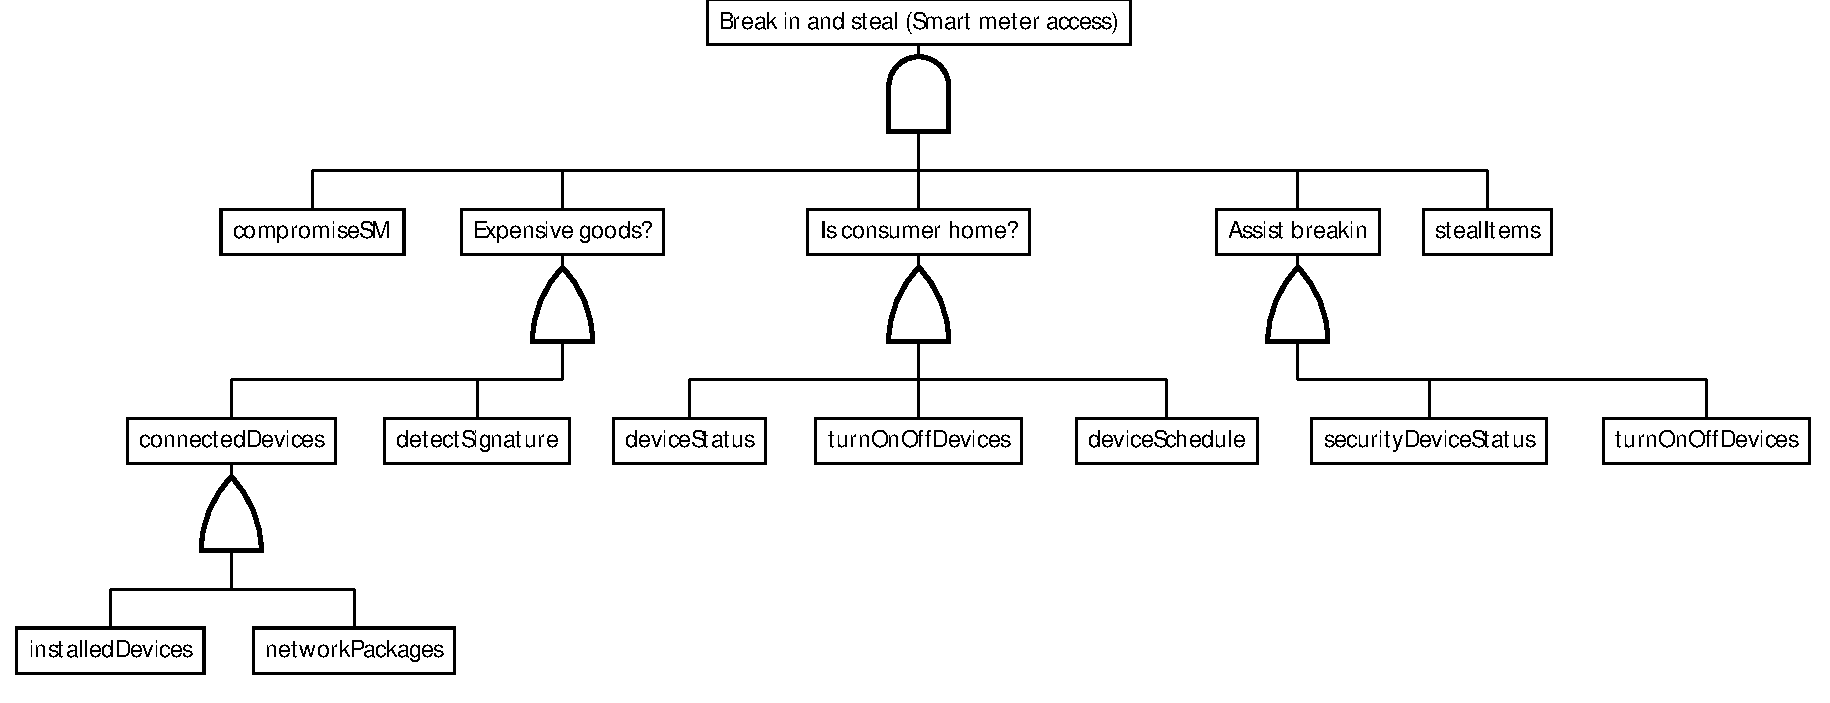
\includegraphics[width=\textwidth]{graphviz/burglarSM.pdf}
\caption{A burglar attacking the consumer using the smart meter.}
\label{attacktree:burglar:sm}
\end{figure}

\cleardoublepage
\KOMAoptions{paper=A4,pagesize}
\recalctypearea
}


\afterpage{% Insert after the current page
\clearpage
\thispagestyle{plain}
\KOMAoptions{paper=A3,paper=landscape}
\recalctypearea

\begin{figure}
\center
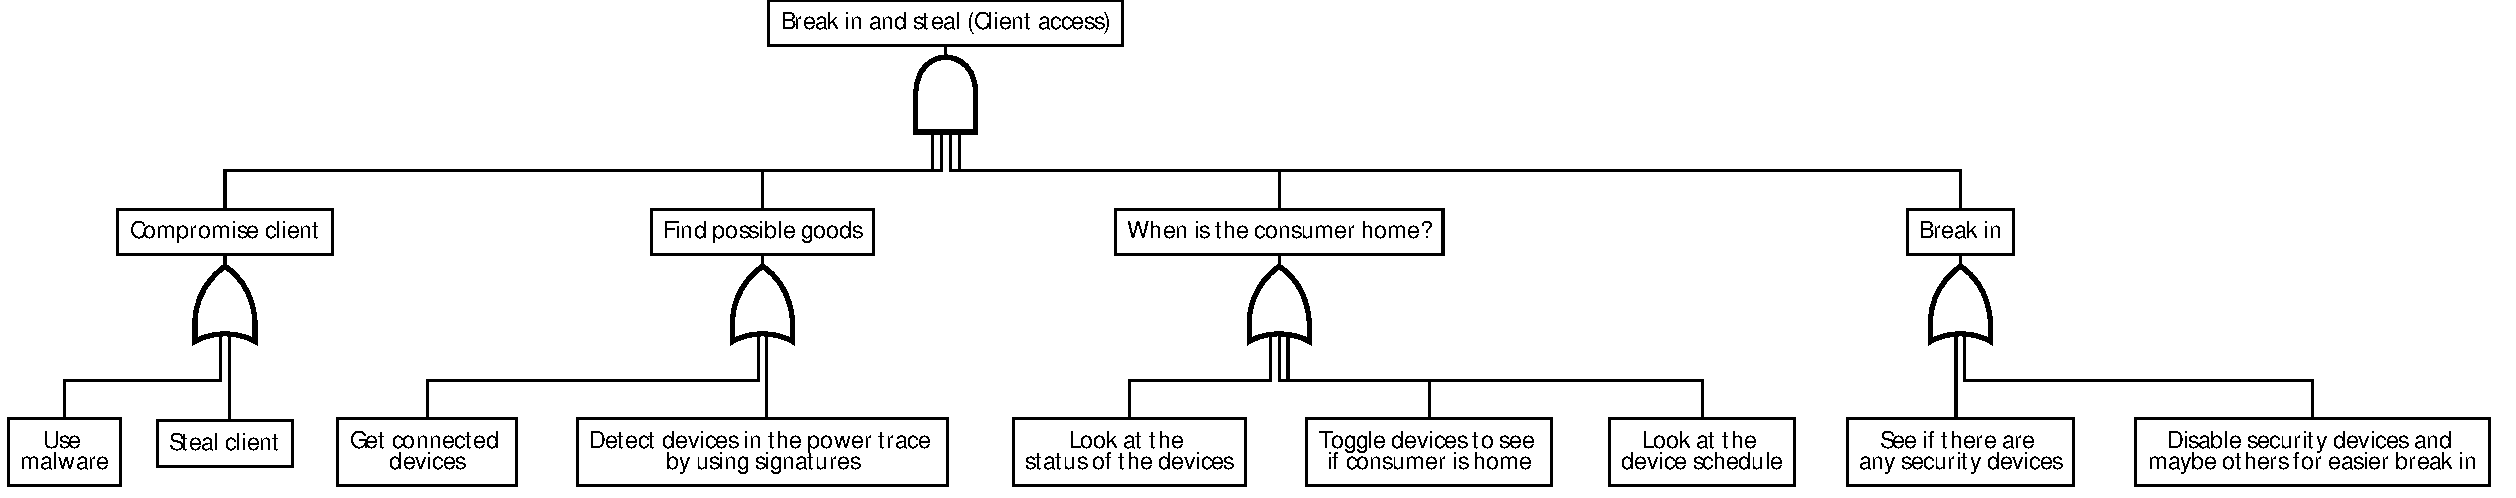
\includegraphics[width=\textwidth]{graphviz/burglarClient.pdf}
\caption{A burglar attacking the consumer using the consumers client.}
\label{attacktree:burglar:client}
\end{figure}

\cleardoublepage
\KOMAoptions{paper=A4,pagesize}
\recalctypearea
}


\afterpage{% Insert after the current page
\clearpage
\thispagestyle{plain}
\KOMAoptions{paper=A3,paper=landscape}
\recalctypearea

\begin{figure}
\center
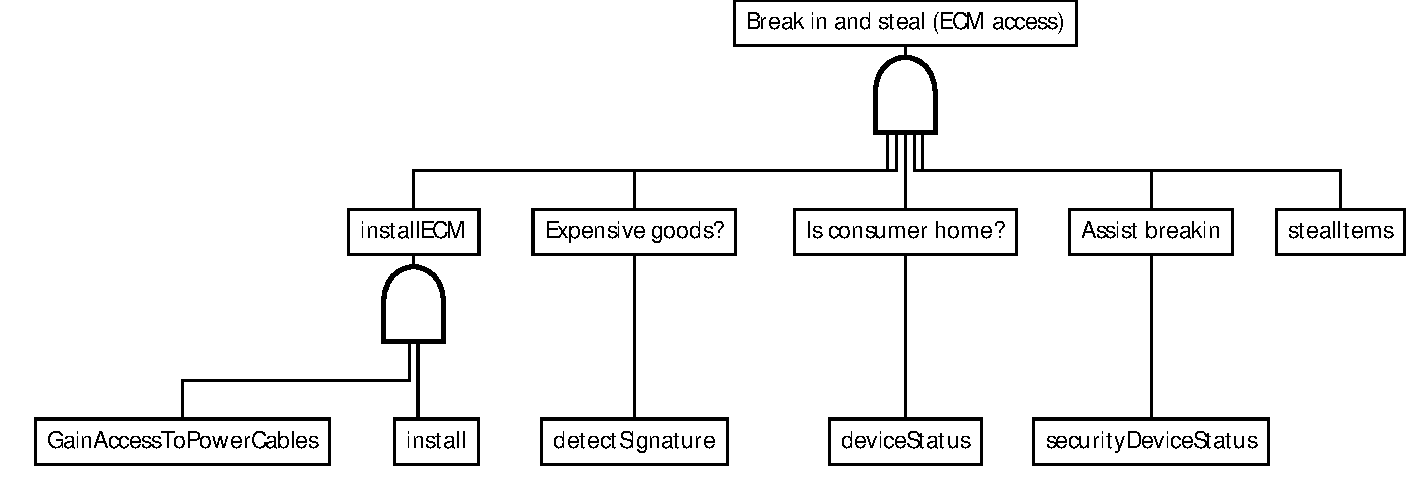
\includegraphics[width=\textwidth]{graphviz/burglarECM.pdf}
\caption{A burglar attacking the consumer using an ECM.}
\label{attacktree:burglar:ecm}
\end{figure}

\cleardoublepage
\KOMAoptions{paper=A4,pagesize}
\recalctypearea
}


\begin{figure}
\center
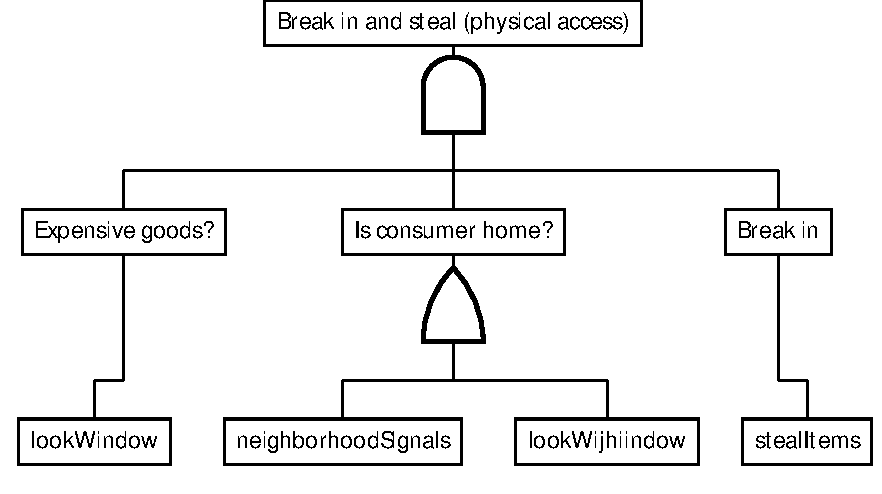
\includegraphics[width=0.75\textwidth]{graphviz/burglarPhysical.pdf}
\caption{A burglar attacking the consumer through physical means.}
\label{attacktree:burglar:physical}
\end{figure}

In the following, the various attacks on the system are described.
As the attacks are similar in structure they are described in terms of their difference.
The structure consists of an initial step where the burglar gains access to information.
Then a step to determine which valuable items the consumer has and a step to determine if the consumer is home.
The final step in the attack is stealing the consumer's valuables.

\subsection{Gaining access}
In order to access information about the power consumption of the consumer, the burglar needs to gain access to either the smart meter, a consumer device that controls the smart meter, or install an ECM unit (see \cref{ecm}).
The following will discuss the subtrees concerning these access methods.

\subsubsection{Compromising the smart meter}\label{compromise:SM}

\begin{figure}[H]
\center
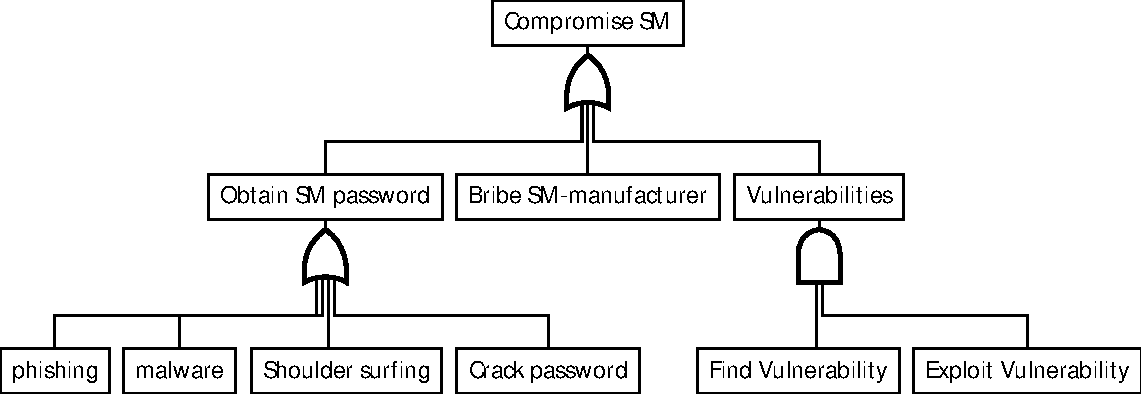
\includegraphics[width=\textwidth]{graphviz/CompromiseSM.pdf}
\caption{Subtree for compromising the smart meter.}
\label{attacktree:compromiseSM}
\end{figure}

There are three general ways of compromising the smart meter.
The subtree can be seen in \cref{attacktree:compromiseSM}.
First of all, if you have the password for logging it is possible to access the same information as the consumer is.
There are a couple of methods for gettings one's hands on this password. 
\begin{description}
	\item[Phishing] The burglar can attempt to get the password directly from the consumer by posing as the electrical company or similar. Phishing will be discussed in \cref{attack:phishing}
	\item [Shoulder surfing] If the burglar has the possibility of watching the consumer in a context where he enters his password, he can retrieve the password, or hints about the password, by shoulder surfing. 
	Shoulder surfing can also lead to information about the consumer, or the smart meter, that will help the consumer carrying out one of the other option, such as finding the brand of smart meter for constructing a phishing email.
	Shoulder surfing will be discussed in \cref{attack:shoulder}
	\item [Malware] It is also possible to get the password by infecting a client device of the consumer with some malware.
  This piece of malware can either send the password back to the burglar or provide access to the system.
  Malware will be discussed in \cref{attack:malware}
	\item [Crack password] If the other options do not amount to anything, the burglar can resort to cracking the password.
	Password cracking will be discussed in \cref{password_cracking}.
\end{description}

The second option is to bribe the smart meter company to make some changes to the firmware that help achieve the goal.
This could be adding a backdoor to the firmware, or to change how the firmware handles consumption data.
This is an effective way of achieving something on a lot of smart meters, as the smart meter manufacturer will push the firmware to a lot of customers.

Another option is to find some vulnerability in the smart meter firmware.
Depending on the vulnerability, the burglar can possibly perform actions that was not intended by the manufacturer.
Other vulnerabilities will make it possible to access the same information as available to the consumer.
An example of a vulnerability is a buffer overflow.
Buffer overflows will be discussed in \cref{attack:bufferoverflow}.
If a buffer overflow is found it may make it possible to run arbitrary code on the smart meter which can possibly open for everything.


\subsubsection{Compromising the client}\label{compromise:client}

\begin{figure}[H]
\center
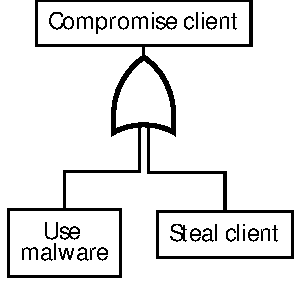
\includegraphics[width=0.35\textwidth]{graphviz/CompromiseClient.pdf}
\caption{Subtree for compromising a client of the consumer.}
\label{attacktree:compromiseClient}
\end{figure}

An alternative point of attack is the client that the consumer uses to control the smart meter.
The subtree for this case can be found in \cref{attacktree:compromiseClient}.
The obvious possibility is to steal the client that the consumer uses.
If the consumer uses a tablet for controlling the smart meter, this can be done when the consumer is at out of the house or at work by ``conventional'' mischievous methods.
Assuming the burglar can overcome the login to the client, he will be able to access the smart meter as if he was the consumer.

Alternatively, the burglar can use malware to gain either the password to the smart meter or access to the client.
This step is similar to the malware item earlier in this section.



\subsubsection{Installing an ECM} \label{compromise:ecm}

\begin{figure}[H]
\center
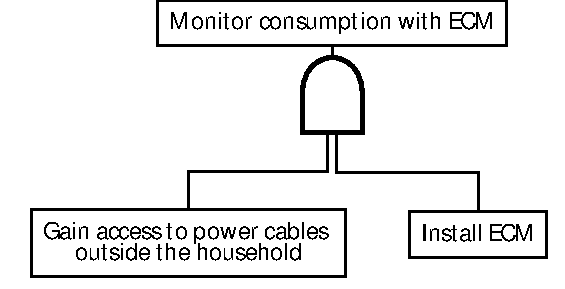
\includegraphics[width=0.6\textwidth]{graphviz/ECM.pdf}
\caption{Subtree for monitoring the consumer with an attached ECM.}
\label{attacktree:ECM}
\end{figure}

If it is not possible for the burglar to get access to the smart meter, or the client, from the outside, he has another option.
An External Consumption Monitor (ECM) is a device that can monitor the consumption of a electricity cable (ECM will be discussed further in \cref{ecm}).
If the burglar can find the incoming power cable and attach such a device, he can get roughly the same data as the consumer gets through his smart meter and therefore he will be able to perform many of the same attacks as with access to the smart meter.

The subtree depicting how to achieve this can be seen in \cref{attacktree:ECM}.


\subsection{Expensive goods}
The first step for the burglar, after gaining access to the system, is to determine if anything is of value in the house. 
The burglar can choose any house he wants and will use the information obtained to determine which house will yield the highest total worth for the least amount of effort.

\paragraph{Physical means}
The physical method is simply to look in through windows of the house and consider what can be seen. 
This method has some obvious shortcomings.
Not everything can be seen from the outside, and in multiple story houses several stories may be impossible to evaluate.
Is is also rather inaccurate -- it may be possible to see a TV, but is it the newest product from this year, or is it an older model that is virtually impossible to sell?

\paragraph{Compromised smart meter or router}
If the burglar has compromised either the smart meter or the internet router of the consumer, he will be able to find out what products are in the home. 
This is possible either through some smart meter database that shows what can be controlled, or through network traffic which can indicate what products are being communicated with.

\paragraph{Power consumption}
If the burglar has access to the power consumption (either smart meter or the ECM), it will be possible to detect product signatures in this data, see \cref{smart_meter_privacy}.
This is difficult and possibly ambiguous, but it may provide pointers on what he can expect to find.

\subsection{Is the consumer at home?}
When the burglar decides on a home to be his target, he needs to plan when to break in.
Before doing that he needs information about when the consumer is home.

\paragraph{Physical means}
The burglar can use some physical methods to determine if the consumer is at home.
He can look through the windows to check for activity in the house.	
This technique is not guaranteed to show that nobody is home, but if there is activity the burglar can be sure that someone is at home.
Over a longer period of time this technique can provide information about the habits and work hours of the consumer, making it easier to plan when to break in and when to be out again.

Another technique is to put indicators in the neighbourhood.
This could be small signs on the mailbox, a can behind the tire of a car, or a knocked over bike.
The purpose of these subtle indicators is to find out if the home is empty for a longer period of time.
If the consumer is home it is likely that he will erect the bike and/or remove the mark from the mailbox.
If all indicators are left untouched it is likely that the consumer is not at home.
This technique is very fast to apply to a consumer's home and can thus easily be applied to multiple homes.

\paragraph{Compromised smart meter}
Having access to the smart meter may gain access to schedule information which can be an indicator of when the consumer is at home.
If the consumer schedules laundering during the night it may indicate that he plans to be home shortly after after the laundering has ended.
The schedule may also provide information about work hours of the consumer, making it possible for the burglar to plan the break in.

Having control over the smart meter also provides the power to turn devices on or off.
The burglar can use this to reinforce any suspicion he has that the consumer is home or not.
If he thinks that the TV is turned on by some timer mechanism he can force it to turn off.
If the consumer is really at home he will probably turn it on again.
Provided that this action must be done manually, this is a sure-fire proof that the consumer is at home.
Another test could be to turn the stereo on and put the volume to an abnormally high level.
If the consumer does not react to this, he is either sleeping very tight or not at home.

\paragraph{Power consumption}
If the burglar has access to the smart meter or an ECM (External Consumption Meter) he has some options that can help him determine if the consumer is at home.

From the power consumption it is possible to determine which devices are currently on. 
If the TV is turned on and off in irregular intervals (timers exist that can turn devices on and off at predetermined intervals), it is an indicator that the consumer is home.

\subsection{Break in}
When the burglar feels confident that he wants to break in to the house, he can use the smart meter for some additional help.
The smart meter can provide information about the security status of the house.

If there is a security alarm or camera, this will be visible on the smart meter by the same techniques mentioned in the ``Expensive goods'' subtree -- either in the consumption data, network data, or smart meter database.
If the consumer has some security devices installed, the burglar can turn them off entirely and make the break in easier before he even enters the property.

The last step is to steal all the expensive goods in the house of the consumer.
The smart meter (as well as surveillance) might provide the burglar with information that lets him know when the consumer is usually home, and he therefore knows when to be out in order to not get caught.
